\section{Arquitectura}

\subsection{ARS}

\par Primero vamos a presentar la arquitectura del core de nuestro sistema (ARS), es decir de la parte que se encarga de realizar todas las operaciones sobre los datos (ver figura \ref{fig:dia_cyc_core}). \\

\par El encargado de recibir los datos que ingresan al sistema ARS es el \textit{Receptor de mediciones}. A este componente le llegan las mediciones provenientes de los sensores y las publica en un bus, al cual está suscripto el \textit{Procesador de mediciones}. El procesador es el encargado de realizar el trabajo de limpieza y agregación de los datos, para luego colocarlos en el \textit{Repositorio de datos históricos} (más adelante haremos zoom sobre este componente para ver en detalle cómo funciona). \\

\par Paralelamente hay un componente llamado \textit{Detector de anomalías}, quien lee los datos ingresados en el repositorio y les aplica algoritmos de big data y machine learning con el propósito de detectar valores anómalos en las mediciones procesadas (para detectarlos también realiza comparaciones con los datos del simulador \textit{SimOil}). Al encontrar un dato no esperado, le envía un call asincrónico al \textit{Activador de alarmas} con toda la información correspondiente a la anomalía, y éste procede a escribir el evento en el \textit{Repositorio de eventos}, al mismo tiempo que se lo comunica al \textit{Enviador de avisos de alarma}. El enviador es el encargado de enviar la notificación a través de una interfaz SMS. Notar que está conectado a un timer y a un repositorio de mensajes pendientes, esto es porque la interfaz SMS no siempre está disponible, y el componente debe reintentar los envíos de mensajes cada cierto tiempo. \\

\par El \textit{Informador de nuevos datos} es el componente encargado de comunicarle al ente regulador por mail que hay nuevos datos en el ARS. Para esto está conectado a un timer, de esta manera puede revisar los cambios en el repositorio de datos históricos cada cierto tiempo. Vale aclarar de que el mail que se envía es solo informativo, es decir, no contiene los datos nuevos sino que es solo un aviso (esto es porque el servicio de mail no es seguro, y sería riesgoso para mantener la seguridad del sistema enviar toda la información de las mediciones). Además, enviar los datos puede ser muy poco performante ya que el peso del mail con toda la información puede llegar a ser muy grande. \\

\par Por otro lado, como es crucial para nuestra arquitectura tener un repositorio de datos históricos, decidimos darle disponibilidad mediante la realización de un backup. Para esto hay un componente (\textit{Backups updater}) que realiza el backup en los repositorios de backup 1 y 2. En el caso en que el repositorio principal deje de estar disponible, todos los componentes que interactúan con él pasarán a apuntar a alguno de los backups (para que el usuario no detecte la falla), mientras que otro componente, el \textit{Backup restorer}, se encargará de restaurar los datos. \\

\par Los componentes \textit{Buscador de datos históricos}, \textit{Buscador de eventos} y \textit{Archivador de revisión} los explicaremos más adelante dado que se relacionan con las interfaces de usuario.

\newpage
\begin{figure}[H]
  \centering
  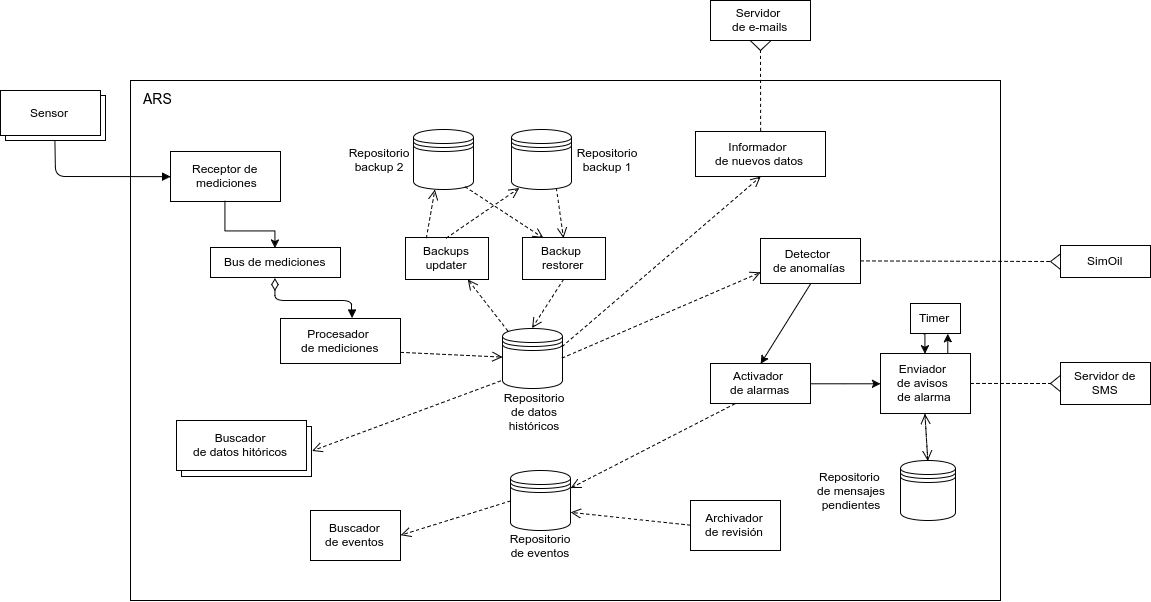
\includegraphics[angle=-90,scale=0.52]{imagenes/diagramas/core.png}
  \caption{Diagrama de componentes y conectores que muestra la estructura del ARS y la interacción entre los componentes mas significativos.}
  \label{fig:dia_cyc_core}
\end{figure}
\newpage

\subsection{Procesador de Mediciones}

En la figura \ref{fig:proc_med} podemos observar en detalle el componente Procesador de mediciones (perteneciente al ARS). El mismo posee dos etapas. La primera es la encargada de limpiar los datos recibidos y para ello existen múltiples \textit{Limpiadores de datos}, suscriptos a un Bus de mediciones. Cada uno de los limpiadores se suscribe al tipo de evento que es capaz de procesar (datos de temperatura o presión). Una vez superada esta instancia del proceso, se almacenan los datos en el \textit{Repositorio de datos limpios}. \\

\par Luego, varios \textit{Agregadores de mediciones} leen los datos del repositorio, ya sean de temperatura o presión, según la frecuencia seteada por el Timer. Una vez leídos los datos, el mismo componente los borra del repositorio. El objetivo de esto es transformar los datos de alta frecuencia (provenientes de los sensores) en intervalos manejables de 15 minutos. Al finalizar la agregación, las mediciones procesadas son almacenadas en el Repositorio de datos históricos.

\begin{figure}[H]
  \begin{subfigure}{\textwidth}
    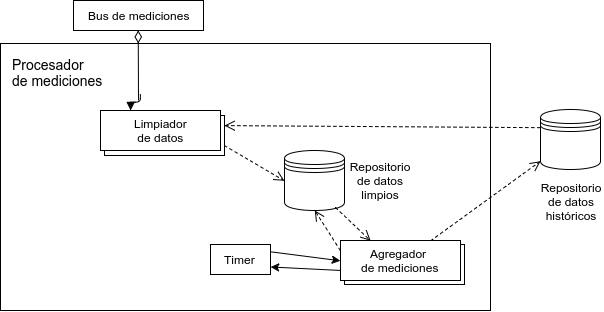
\includegraphics[width=\textwidth]{imagenes/diagramas/procesadorDeMediciones.png}
  \end{subfigure}
  \caption{Diagrama de componentes y conectores del Procesador de mediciones}
  \label{fig:proc_med}
\end{figure}



\subsection{Relación de ARS con las UI en clientes}

\par Las funcionalidades disponibles de nuestro sistema ARS desde el punto de vista de la interfaz de usuario son: monitoreo de datos, visualizar la lista de eventos y revisar los mismos. En todos los casos se necesita que el cliente se comunique con el servidor.

\begin{itemize}
    \item \textbf{Monitor de datos:} El usuario ingresa a la pantalla de monitoreo y el componente \textit{UI monitor de datos} le envía un mensaje asincrónico al \textit{Solicitador de datos} para pedirle las últimas mediciones tomadas. Al recibir esta petición, lee en el \textit{Repositorio de sesión} las credenciales de sesión actual y le envía un mensaje al componente \textit{UI monitor de datos} para avisarle que recibió su solicitud y que la está procesando. El \textit{Solicitador de datos} se comunica de manera segura (ya que viajan credenciales) con el \textit{Buscador de datos históricos} (que se encuentra en el servidor ARS). Es importante aclarar que le pide una cantidad limitada de datos. Una vez que un \textit{Buscador de datos históricos} recibe una petición, valida que el usuario posea los permisos necesarios para acceder a los datos pedidos (por medio del \textit{Repositorio de perfiles de usuarios y sesiones}). \\
    Si el usuario no posee permisos (o su sesión no es válida), el buscador le responde al solicitador acceso denegado. En el caso de que el usuario posea los permisos necesarios, el \textit{Buscador de datos históricos} lee desde el \textit{Repositorio histórico de datos} los datos requeridos para luego enviárselos al \textit{Pulicitador de datos}. Una vez que este recibe la respuesta, se la comunica a la \textit{UI monitor de datos} para que los muestre. Como es una herramienta de monitoreo se necesita que con el correr del tiempo se muestren nuevos datos sin la solicitud expresa del usuario. Por esta razón, incluimos un componente llamado \textit{Timer} para que luego de un tiempo configurado le avise al \textit{Solicitador de datos} que debe pedir nuevos datos. Al recibir este aviso, realiza un nuevo pedido al \textit{Buscador de datos históricos} indicando que se quieren obtener solo datos con fecha mayor al último pedido.
    \item \textbf{Visualizar la lista de eventos:} El usuario accede a la pantalla de listar eventos y el componente UI listado de eventos le envía un mensaje asincrónico al solicitador de eventos y éste le envía otro mensaje asincrónico para avisarle que recibió la solicitud. El solicitador de eventos lee los datos del usuario en el repositorio de sesión y luego establece una conexión segura con el buscador de eventos para solicitarle la lista de eventos. El buscador de eventos lee el repositorio de usuarios, roles y sesiones para validar los datos de acceso y luego el repositorio de eventos para pedir la lista de eventos. El buscador de eventos le envía la lista al solicitador de eventos para que éste se lo reenvíe a la interfaz de usuario. \\
    De manera opcional, el usuario puede seleccionar un evento en particular. En ese caso, UI listado de eventos le envía un mensaje sincrónico al selector de evento con el evento elegido para que lo almacene en el Repositorio de evento seleccionado.
    \item \textbf{Visualizar detalle del evento seleccionado:} Una vez que el usuario logueado está en la pantalla de visualización de un evento en particular, la \textit{UI detalle del evento} por medio de un call asincrónico le indica al \textit{Solicitador de evento} que busque en el \textit{Repositorio de evento seleccionado} (después de validar la sesión por medio de la lectura del \textit{Repositorio de sesión}) cuál es el evento a mostrar. Los datos del mismo son enviados por otro call asincrónico a la misma UI, que sabe como renderizar la información requerida.
    \item \textbf{Revisión de eventos:} En la pantalla de revisión de evento el usuario puede informar la acción realizada o bien, un falso positivo. La interfaz de usuario de revisión de evento le envía un call sincrónico con el resultado del evento para que el informador de revisión lea el repositorio de sesión y luego se lo pase al archivador de revisión. El archivador de sesión valida los datos de usuario y escribe en el repositorio de eventos la medida tomada o el falso positivo.
\end{itemize}

\begin{figure}[H]
  \begin{subfigure}{\textwidth}
    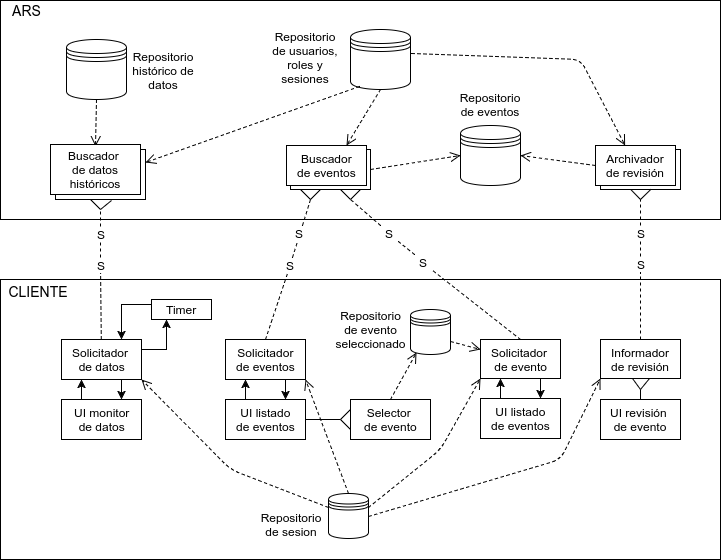
\includegraphics[width=\textwidth]{imagenes/diagramas/interaccionConClientes.png}
  \end{subfigure}
  \label{}
  \caption{}
\end{figure}

\subsection{Autenticación y creación de sesiones}

\par A continuación pasaremos a explicar los procesos de autenticación, creación de sesión y finalización de sesión. Estos procesos se observan en el diagrama de componentes y conectores de la figura \ref{fig:dia_cyc_autenticacion}.\\

\par El proceso de autenticación con el sistema ARS inicia cuando una persona ingresa sus datos de usuario y contraseña en la \textit{UI Login}, que envía estos datos al \textit{Iniciador de login} y se queda esperando la respuesta. Éste, por su parte, inicia una conexión segura con el \textit{Validador de usuarios y contraseñas} (dentro del sistema ARS) para enviarle la petición junto con los datos sensibles de autenticación. Al recibir la petición, el componente \textit{Validador de usuarios y contraseñas} se conecta con el \textit{Hasher}, le envía la contraseña y espera a que sea procesada y devuelta. Una vez obtenido el hash de la contraseña, el componente \textit{Validador de usuarios y contraseñas} corrobora en el \textit{Repositorio de usuarios y contraseñas hasheadas} que exista un usuario que corresponda a esos valores. \\

\par En caso que no se encuentre el usuario corespondiente, se responde al \textit{Iniciador de sesión} con un error que indica que alguno de los datos ingresados es incorrecto. Este componente responde de la misma manera a la \textit{UI Login} para que muestre el error. En caso de que el componente \textit{Validador de usuarios y contraseñas} encuentre al usuario que corresponde a los valores buscados, le pide al \textit{Creador de sesiones} que genere una nueva sesión para este usuario. Luego de generar la sesión, el \textit{Creador de sesiones} la guarda en el \textit{Repositorio de perfiles de usuarios y sesiones} y responde al \textit{Validador de usuarios y contraseñas} con esta nueva sesión. Para finalizar, se envía esta nueva sesión al \textit{Iniciador de sesión}, quien la almacena en el \textit{Repositorio de sesión} y le comunica a la \textit{UI Login} que se ha conseguido iniciar sesión correctamente.\\

\par Para el caso del cierre de sesión, cualquier componente dentro de \textit{UI} (donde se incluyen las interfaces para usuarios autenticados) puede enviar una petición al \textit{Finalizador de sesión}, quien inicia una conexión segura con el componente \textit{Borrador de sesión} (dentro del sistema ARS) y le comunica que quiere borrar la sesión. Es importante mencionar que la conexión debe ser segura porque un intermediario podría hacerse pasar por el sistema ARS, contestar que se procesó la petición y continuar utilizando esta sesión válida con acceso a datos sensibles del sistema. El componente \textit{Borrador de sesión} valida la sesión con el \textit{Repositorio de perfiles de usuarios y sesiones}, la marca como finalizada y envía la respuesta al \textit{Finalizador de sesión}. Por último, este componente borra la sesión que se encontraba almacenada en el \textit{Repositorio de sesión} y comunica a quien inició la petición que se procesó el pedido con éxito.

\begin{figure}[H]
  \begin{subfigure}{\textwidth}
    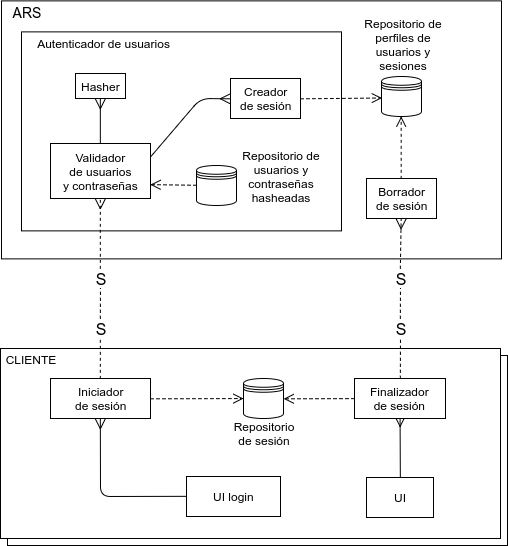
\includegraphics[width=\textwidth]{imagenes/diagramas/loginYLogout.png}
  \end{subfigure}
  \caption{Diagrama de componentes y conectores que participan de los procesos de autenticación y finalización de sesiones.}
  \label{fig:dia_cyc_autenticacion}
\end{figure}



\subsection{Estructura general}

Finalmente, y abstrayéndonos de los detalles, los componentes que interactúan en todo el sistema se observan en la figura \ref{fig:general}.

\begin{figure}[H]
  \begin{subfigure}{\textwidth}
    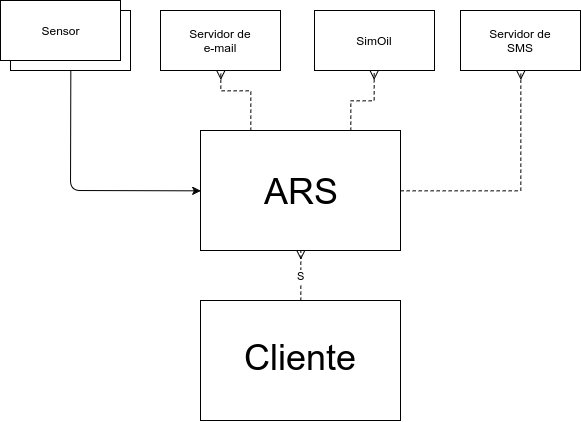
\includegraphics[width=\textwidth]{imagenes/diagramas/general.png}
  \end{subfigure}
  \caption{Diagrama general del sistema}
  \label{fig:general}
\end{figure}

Todo el sistema ARS va a estar instalado en el Ministerio de Energía, junto con el de SimOil, y los sensores van a estar ubicados en el yacimiento.


\newpage